\chapter{Nanofabrication}
\label{sec:fab}
In this appendix, I will briefly outline the steps followed to fabricate the devices presented in this thesis.
Although there are several types of devices presented, including quantum dots, nanowire devices, and Hall bars,
in each case the techniques used for each chip are adapted from the steps laid out below. The significant differences
in cleanroom tooling and safety protocols in each cleanroom mean that several procedures will likely need to be
adapted to gain similar results, however, where possible I've tried to include all the details that would be necessary
to tailor the process to your cleanroom.

\section{Fabrication Overviews}
\label{sec:fab_overview}

\subsection{Quantum Dot Nanofabrication}
\begin{enumerate}
    \item \textbf{Cleave Chips} (Sec.~\ref{sec:cleave})
    \item \textbf{Gallium Removal}: Remove gallium on the backside of wafer. (Sec.~\ref{sec:garem})
    \item \textbf{Chip Clean and Bake}: Remove any organic solvents and adsorbed moisture. (Sec.~\ref{sec:clean})
    \item \textbf{Alignment Mark Deposition}: Deposit TiAu alignment marks which will be our reference for all future fab steps. (Sec.~\ref{sec:metaldep})
    \item \textbf{Mesa Etch}: Define the active region of the device by etching away the 2DEG using a dilute \ce{H3PO4} solution. (Sec.~\ref{sec:mesaetch})
    \item \textbf{Ohmics Deposition}: Deposit AuGe ohmics and anneal into wafer. This step should be performed as soon as possible after the etch, preferrably on the same day. (Sec.~\ref{sec:ohmics})
    \item \textbf{Ohmic Contact Deposition}: Deposit bondpads for ohmic contacts. (Sec.~\ref{sec:metaldep})
    \item \textbf{Global Oxide Deposition}: Deposit a global \ce{Al2O3} or \ce{HfO2} oxide using ALD as a insulating barrier. (Sec.~\ref{sec:ald})
    \item \textbf{Gate Deposition}: Deposit surface gate pattern. (Sec.~\ref{sec:metaldep})
    \item \textbf{Gate Contact Deposition}: Deposit bondpads for surface gates. (Sec.~\ref{sec:metaldep})
\end{enumerate}

\subsection{InAs Hall Bar Nanofabrication}
\begin{enumerate}
    \item \textbf{Cleave Chips} (Sec.~\ref{sec:cleave})
    \item \textbf{Chip Clean and Bake}: Remove any organic solvents and adsorbed moisture. (Sec.~\ref{sec:clean})
    \item \textbf{Mesa Etch}: Define the active region of the device by etching away the 2DEG. Note that if Al is grown on the surface, this must be removed (Sec.~\ref{sec:transene}) prior to the mesa etch. (Sec.~\ref{sec:mesaetch})
    \item \textbf{Al Removal}: Etch away excess Al from the surface of the hall bar. (Sec.~\ref{sec:transene})
    \item \textbf{Global Oxide Deposition}: Deposit a global \ce{Al2O3} or \ce{HfO2} oxide using ALD as a insulating barrier. (Sec.~\ref{sec:ald})
    \item \textbf{Gate Deposition}: Deposit surface gate pattern. (Sec.~\ref{sec:metaldep})
\end{enumerate}

\subsection{GaAs Hall Bar and Circulator Nanofabrication}
\begin{enumerate}
    \item \textbf{Cleave Chips} (Sec.~\ref{sec:cleave})
    \item \textbf{Gallium Removal}: Remove gallium on the backside of wafer. (Sec.~\ref{sec:garem})
    \item \textbf{Chip Clean and Bake}: Remove any organic solvents and adsorbed moisture. (Sec.~\ref{sec:clean})
    \item \textbf{Mesa Etch}: Define the active region of the device by etching away the 2DEG using a dilute \ce{H3PO4} solution. (Sec.~\ref{sec:mesaetch})
    \item \textbf{Ohmics Deposition}: Deposit AuGe ohmics and anneal into wafer. This step should be performed as soon as possible after the etch, preferrably on the same day. (Sec.~\ref{sec:ohmics})
    \item \textbf{Gate Contact Deposition}: Deposit bondpads for surface gates. (Sec.~\ref{sec:metaldep})
\end{enumerate}

\section{Detailed Process Recipes}
\subsection{Cleave Chips}
\label{sec:cleave}
In the following section, I will only describe the process for manual cleaving of chips using a diamond tip pen.
For more precise jobs, I recommend the use of a scribing tool which can better align and scribe chips.
For most III-V materials (100 orientation), you will only be able to scribe parallel to or perpendicular to the wafer flat.
Note that all steps should be performed on a cleanroom wipe which is to be disposed of in a contaminated (III-V) waste bin
once the process is complete, due to the hazardous nature of III-V materials.
\begin{enumerate}
    \item Find wafer in fabrication logbook. Note previously scribed pieces and orientation. Select a piece to scribe. Record selected chip orientation and position in fabrication logbook.
    \item Line up the chip with the edge of a metal ruler. Using a diamond pen, make a small scratch (< \SI{1}{\milli\meter}) to the wafer edge.
    \item Balance the chip on the edge of a glass side with the scratch aligned to the edge of the slide.
    \item Press the overhanging section of the chip with filter paper or a cleanroom wipe to cleave the chip. The cleave should be clean and along the scratch direction.
    \item Choose a corner of the chip as a reference for future steps. Make a drawing of the scratches/features of the chip relative to the corner in the fabrication of logbook. Note the wafer orientation relative to the chip for future reference.
    \item Put contaminated filter paper/wipes in the contaminated wase bin, and glass slides into the sharps disposal.
\end{enumerate}

\subsection{Gallium Removal}
\label{sec:garem}
Ga metal is used as a sticking layer and thermal contact in the MBE chamber during heterostructure growth. When wafers
arrive from growers they often have this sticking layer still on their backsides, which must be removed before further processing
as it has a melting point of \SI{29}{\celsius} and tends to contaminate process equipment and coat the surface of glassware.
We use the low melting point of Ga to physically remove it using q-tips followed by an optional \ce{HCl} dip to etch away any remnants.
The \ce{HCl} dip is useful to obtain the lowest possible ohmic resistances and is used more for Hall chips than quantum dots.
\begin{enumerate}
    \item Heat a small amount of NMP to \SI{80}{\celsius} in the designated NMP-(Gallium) beaker. It should be sufficiently full to cover the chip that will be placed in step 3. Prepare a small amount of NMP in an NMP-(Clean) beaker.
    \item Deposit 1-2 drops of PMMA onto the bottom third of a clean glass slide.
    \item Carefully place the GaAs chip facedown on the PMMA droplet, attempting to keep the back dry and free of resist.
    \item Place the glass slide on a \SI{95}{\celsius} hotplate for at least \SI{1}{\minute}.
    \item Using a cleanroom q-tip, gently wipe the Ga from the back of the chip, replacing the q-tip as necessary. Ensure that the chip does not move during this process as movement may damage the chip surface. The chip may be placed on the hotplate for an extra \SIrange{20}{30}{\second} if the Ga has dried.
    \item Place the glass slide in the heated NMP-(Gallium) beaker such that it is covered. Gently nudge the chip after \SI{30}{\second} until it is free of the slide and discard. Transfer the chip into the second NMP-(Clean) beaker.
    \item \textbf{Optional:} If at this point the gallium is sufficiently removed we may proceed directly to the chip clean and bake (Sec.~\ref{sec:clean}). Otherwise, transfer the chip to an IPA-(Clean) beaker with a small amount of IPA and sonicate for \SI{1}{\minute}.
    \item Spin and bake AZ6612, PMMA, or a similar photoresist (Sec.~\ref{sec:spin}). In general, ZEP or CZAR should be avoided for acid etches.
    \item Stir the chip in a \SI{37}{\percent} \ce{HCl} solution for \SIrange{2}{3}{\minute}.
    \item Rinse the chip in distilled \ce{H2O} for \SI{30}{\second}.
    \item Proceed to chip clean and bake (Sec.~\ref{sec:clean})
\end{enumerate}

\subsection{Clean and Bake}
\label{sec:clean}
The clean and bake step is used to remove any surface contaminants that may have been introduced in shipping and handling, as well as to
remove any surface moisture. Each solvent step should include some sonication during the \SI{5}{\minute} soak. Sonication may be performed for
the full \SI{5}{\minute} if desired. Tweezers should be washed in between each transfer step to prevent cross-contamination.

\note{NMP easily damages Al if the solvent has absorbed any moisture from the air. For materials with thin-film epitaxially grown Al, use an alternative solvent such as 1,3-Dioxolane.}

\begin{enumerate}
    \item Place chip, face-up, in a small amount of NMP at \SI{80}{\celsius}, in an NMP-(Clean) beaker for at least \SI{5}{\minute}, with sonication.
    \item Transfer the chip to Acetone in an Acetone-(Clean) beaker for at least \SI{5}{\minute}, with sonication.
    \item Transfer the chip to IPA in an IPA-(Clean) beaker for at least \SI{5}{\minute}, with sonication.
    \item Remove the chip from the IPA and dry with nitrogen on a fresh cleanroom wipe.
    \item Bake the chip at \SI{200}{\celsius} for \SI{5}{\minute}.
\end{enumerate}

\subsection{Resist Strip}
\label{sec:strip}
This process is used to strip resist of the surface of a chip, either due to a failed processing step or after a mesa etch (Sec.~\ref{sec:mesaetch}).
In the case that the strip is being performed during spinning and before the resist has been baked, it is usually sufficient to perform a quick \SI{30}{\second}
Acetone/NMP dip rather than the longer times prescribed below, as the resist will not be hardened. Sonication may be used to assist with the strip
as long as fine gates have not been evaporated. Otherwise, sonication often damages these gates.

\note{ZEP, CZAR and other styrene-based resists are \emph{NOT} compatible with Acetone. For these samples, NMP or an alternative solvent must be used.}

\note{NMP easily damages Al if the solvent has absorbed any moisture from the air. For materials with thin-film epitaxially grown Al, use an alternative solvent such as 1,3-Dioxolane.}

\begin{enumerate}
    \item Place chip, face-up, in a small amount of NMP at \SI{80}{\celsius}, in an NMP-(Clean) beaker, or Acetone in an Acetone-(Clean) beaker for at least \SI{3}{\minute}.
    \item Transfer the chip to IPA in an IPA-(Clean) beaker for at least \SI{30}{\second}.
    \item Remove the chip from the IPA and dry with nitrogen on a fresh cleanroom wipe.
\end{enumerate}

\newcommand{\spinunits}{(\si{\rpm})-(\si{\second})-(\si{\rpm\per\second})}
\subsection{Resist Spin}
\label{sec:spin}

\begin{table}
    \centering
    \hspace*{-1cm}
    \begin{tabular}{lllll}
        \toprule
        Process                                  & PMMA A3     & ZEP520A       & AZ6612       & LOR 5B\\
        \midrule
        Step 1 \spinunits                        & 500-5-1000   & 500-5-1000   & 500-5-1000   & 500-5-1000   \\
        Step 2 \spinunits                        & 9000-5-4000  & 9000-5-4000  & 10000-20-4000& 10000-4-4000 \\
        Step 3 \spinunits                        & 4000-45-4000 & 4000-120-4000& 4000-20-4000 & 4000-60-4000 \\
        Bake (\si{\celsius})-(\si{\second})      & 180-60       & 180-120      & 95-60        & 170-300      \\
        Approx. Thickness (\si{\nano\meter})     & 80           & 220          & 800 - 1000   & 600 - 800    \\
        \bottomrule
    \end{tabular}
    \hspace*{-1cm}
    \caption[Spin recipes for various resists]
    {Spin recipes for various resists. Each step gives a spin speed, a spin time, and an acceleration, separated by dashes.
    Thicknesses quoted are approximate and will vary depending on chip size and resist age and temperature.}
    \label{tab:spin}
\end{table}

\begin{figure}
    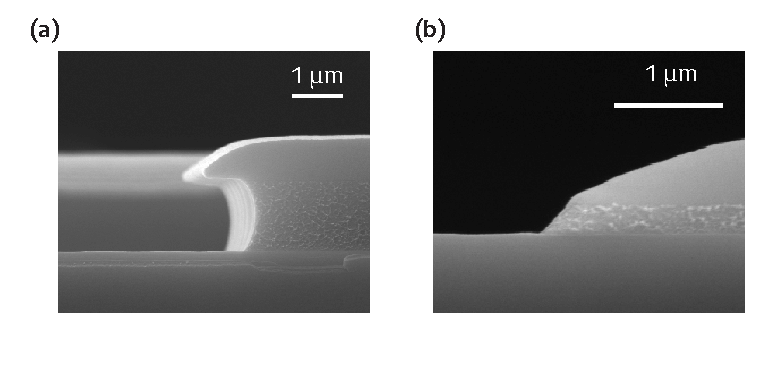
\includegraphics[width=0.85\linewidth]{resistedge}
    \caption[Edge profiles of two resists]
    {\label{fig:resistedge}Edge profiles of LOR 20B/AZ6612 (a) or LOR 5A/AZ6612 (b). The left image shows a significant undercut,
    suitable for deposition of thick metal layers, while the right image shows a smooth edge profile suitable for etching, and caused
    by the low solubility of LOR 5A relative to exposed AZ6612 in MIF300 developer. }
\end{figure}

Spinning resist aims to create a uniform thin film of a photoresist or electron-beam resist. Depending on the sort of process we wish
to run, with the developed resist, we may have different requirements for the edge profile. For evaporation of a metal stack with a
liftoff process, we aim to create an undercut such that there is a break in the metal, with a height larger than the metal thickness we wish to evaporate. This can
be achieved using a single, thick resist layer, which will, in general, have an undercut profile due to the scattering of electrons or light through the resist, or by
the use of a bilayer resist stack, with a soluble polymer such as LOR-B or MMA as the underlayer. An example of a suitable undercut is shown in Fig.~\ref{fig:resistedge} (a).

For an acid etch, we would, in general, prefer a smooth edge profile with no undercut to ensure the continuous flow of fresh acid over the
surface of the wafer and to ensure that acid is easily rinsed away once the etch is complete. This is achieved by a post-development bake which will reflow resist at the edges of the developed region, and re-adhere resist to the surface of the wafer. An example of a
smooth edge profile is shown in Fig.~\ref{fig:resistedge} (b).

Spin parameters for various resists are given in Table~\ref{tab:spin}, which are valid only for small ($2.5 \times 5$ \si{\milli\meter} or $5 \times 5$ \si{\milli\meter}) samples. A high-speed spin is used at the beginning of the spin to minimize the effect of the edge bead, which is a thick region of resist around the edges of the sample caused by surface tension. However, this spin is unsuitable for large samples or wafers and will lead to variable resist thickness across the wafer, or, in the worst case, the wafer being flung from the chuck.

Hint: Squeezing the sides of the rubber puck makes it easier to move chips around. If the chip is not moving after the spin, try squeezing the
puck in a few locations and try again.

\note{If a resist was refrigerated, it must be allowed to warm to room temperature before use. Apart from the viscosity changing with temperature, leading to an unpredictable resist thickness, the cold resist will condense moisture from the air, contaminating the resist for future users.}

\begin{enumerate}
    \item Clean the small rubber puck for chips with Acetone on a cleanroom wipe.
    \item Attach your chip to the small rubber puck. Attempt to center it as much as possible.
    \item Take a few drops of resist with a pipette from the small resist bottle, making sure to not take from the bottom of the bottle.
    \item Dispense 2/3 drops of resist on the surface of the chip and begin the spin as soon as possible.
    \item After the spinning is complete, inspect the chip for a uniform spin. If the spin is not uniform or has picked up particulates, clean the resist (Sec.~\ref{sec:strip}).
    \item Bake the chip for the appropriate time.
    \item Clean the small rubber puck before finishing. Dispose of the pipette, do not replace remaining resist.
\end{enumerate}

\subsection{Resist Develop}
\label{sec:develop}
Developing resist is the process of dissolving exposed (or unexposed for a negative tone resist) regions of resist to create a mask
on the surface of your sample. Depending on the chemistry of the process, the solvent and times vary. For the resist we've used,
development times are summarized in Table~\ref{tab:develop}.
\begin{table}
    \centering
    \hspace*{-1cm}
    \begin{tabular}{llll}
        \toprule
        Process                   & PMMA A3      & ZEP520A      & AZ6612 \\
        \midrule
        Solvent                   & MIBK:IPA 1:3 & o-Xylene     & MIF-300 (TMAH)\\
        Develop Time (\si{second})& 40           & 50           & 50            \\
        Rinse                     & IPA          & MIBK:IPA 1:3 & \ce{H2O}      \\
        Rinse Time (\si{second})  & 20           & 10           & 30            \\
        Second Rinse              & -            & IPA          & -             \\
        Rinse Time (\si{second})  & -            & 10           & -             \\
        \bottomrule
    \end{tabular}
    \hspace*{-1cm}
    \caption[Development recipes for various resists]
    {Development Recipes for various resists.}
    \label{tab:develop}
\end{table}

\note{Plasma ashing samples after the deposition of fine gates has been known to cause static damage.}

\begin{enumerate}
    \item Prepare beakers for each of the solvents necessary for that resist. There should be a dedicated, labeled beaker for each one.
    \item Place chip into each solvent for the requisite time, swirling the chip continuously. Try to move the chip between beakers quickly but smoothly at each step.
    \item Dry the sample with the \ce{N2} blowgun for $\sim \SI{30}{\second}$.
    \item If possible, plasma ash the sample for between \SIrange{5}{25}{\minute} for a photoresist, or \SIrange{20}{60}{\second} for an e-beam resist, immediately before the next processing step.
\end{enumerate}

\subsection{Mesa Etch}
\label{sec:mesaetch}
It is often necessary to define the sections where the 2DEG exists. For Hall measurements, this is used to define the shape of the Hall bar.
For quantum dots, this is used to isolate devices from each other when multiple devices exist on a single chip, and to reduce parasitic
capacitance along readout or pulsing gates. It is also possible to reduce crosstalk between gates by removing the 2DEG below
as much of the length of the gate as possible\cite{doi:10.1063/1.4752863}.

\begin{figure}
    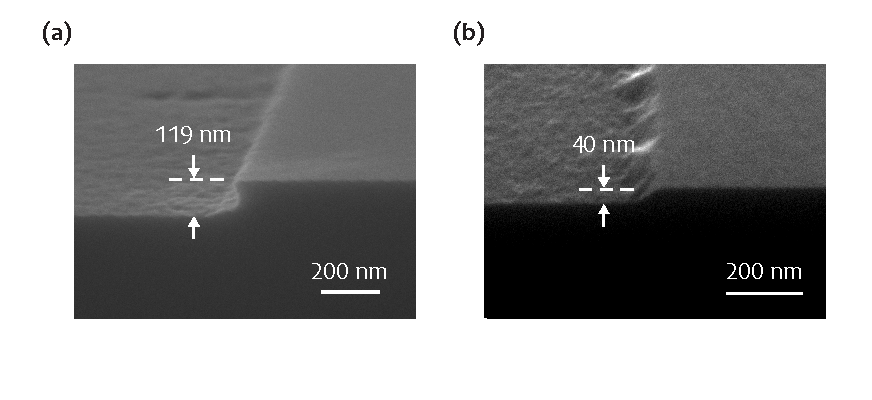
\includegraphics[width=0.85\linewidth]{EtchEdge}
    \caption[Etch profile of \ce{H2SO4} and \ce{H3PO4}]
    {\label{fig:etchedge}A comparison of the etch profiles of \ce{H2SO4} in (a) and \ce{H3PO4} (b). While \ce{H2SO4} leads
    to an anisotropic etch and a significant undercut, the \ce{H3PO4} leads to an isotropic etch and a smooth sidewall.}
\end{figure}

The use of a weaker phosphoric acid solution was chosen after several years of using a sulphuric acid solution as we found that the
strength of the sulphuric acid was leading to an anisotropic etch with a significant undercut. This had, in past devices, led to issues making
continuous gates over the edge of the mesa. The use of phosphoric acid in comparison leads to
an isotropic edge with a smoothly sloping sidewall, making the formation of continuous gates over the mesa edge easier.
A comparison of the etch profiles of \ce{H2SO4} and \ce{H3PO4} is given in Fig.~\ref{fig:etchedge}.

\begin{table}
    \centering
    \begin{tabular}{ll}
        \toprule
        Material & Etch Rate (\si{\angstrom\per\second}) \\
        \midrule
        Intrinsic GaAs & 12.1 \\
        GaAs Heterostructure & 15.9 \\
        InAs Heterostructure & 18.7 \\
        \bottomrule
    \end{tabular}
    \caption[Dilute phosphoric acid (5:1:50 \ce{H3PO4}:\ce{H2O2}:\ce{H2O}) etch rates]
    {Dilute phosphoric acid (5:1:50 \ce{H3PO4}:\ce{H2O2}:\ce{H2O}) etch rates}
    \label{tab:etchratess}
\end{table}

An additional bake is included in the processing after development to remove any undercut that may have developed in the resist during development.
In addition, the drying of the developer has been known to cause the resist to lift from the surface of the wafer near features, which is
repaired by this post-baking step. The addition of this step creates both smoother etch edges and better-controlled edge thicknesses.

\begin{enumerate}
    \item Spin and bake AZ6612, PMMA, or a similar resist (Sec.~\ref{sec:spin}). In general, ZEP or CZAR should be avoided for acid etches.
    \item Expose the mesa pattern using the optical mask aligner or electron-beam lithography. Develop using the appropriate recipe (Sec.~\ref{sec:develop}).
    \item Postbake the resist using the same bake as the initial bake (see Table~\ref{tab:spin}) to remove any undercut and re-adhere the resist to the surface of the chip.
    \item Prepare a solution dilute phosphoric acid solution of \ce{H3PO4}:\ce{H2O2}:\ce{H2O} in a 5:1:50 ratio. Remember that acids should always be added to water, not the other way around. Stir thoroughly with PTFE (acid) tweezers, and leave to thermalize for $\sim \SI{30}{\minute}$.
    \item Measure the resist height with a surface profilometer (Dektak in our case). Record in several locations.
    \item Pour some of the dilute phosphoric acid solution into a small etch beaker. Etch the chip for the appropriate time (use Table~\ref{tab:etchratess} for standard etch rates) using Teflon tweezers and stirring continuously. I usually aim $\sim \SI{10}{\nano\meter}$ below the depth of the 2DEG. Etching too deeply can make it challenging to run gates to the surface of the 2DEG.
    \item Rinse in distilled \ce{H2O} for a minimum of \SI{30}{\second} and dry with nitrogen on a clean wipe.
    \item Measure the new height of the resist using a surface profilometer in the same locations as before. The etch depth is the difference between the two measurements. If the depth is insufficient, repeat steps 5-7.
    \item Strip resist (Sec.~\ref{sec:strip}).
\end{enumerate}

\subsection{Al Etch}
\label{sec:transene}
For InAs devices, aluminum must be selectively etched away to define device geometries. This is accomplished
using a Transene-D based wet etch. This process is highly sensitive to both temperature
and etch time, and hence, care must be taken when performing this step if you wish to achieve reproducible
results. For this reason, a PID controller, glass thermometer, and stirrer are necessary for high quality etches.

For a thin (\SI{8}{\nano\meter}) layer of epitaxially grown Al, we have had success using a \SI{11}{\second} etch
followed by two \SI{11}{\second} \ce{H2O} rinses, however, this process must be optimized for local conditions.

\note{Transene-D will begin to degrade at temperatures above $\sim \SI{50}{\celsius}$. Care must be taken while heating to ensure this temperature is not exceeded, including at the base of the beaker. As such heating must be quite slow.}

\note{Tranene-D oxidizes if stirred too vigorously. The stirrer should be set to the lowest possible speed and should not visibly agitate the surface of the etch solution.}

\begin{enumerate}
    \item Spin and bake AZ6612, PMMA, or a similar resist (Sec.~\ref{sec:spin}). In general, ZEP or CZAR should be avoided for acid etches.
    \item Expose the mesa pattern using the optical mask aligner\ or electron-beam lithography. Develop using the appropriate recipe (Sec.~\ref{sec:develop}).
    \item Postbake the resist using the same bake as the initial bake (see Table~\ref{tab:spin}) to remove any undercut and re-adhere the resist to the surface of the chip.
    \item Prepare a solution of Transene-D, heated to \SI{47.5}{\celsius} with a PID controller, and stirred at low speed. Ensure this temperature is stable before beginning the etch.
    \item Prepare two beakers of DI-water for the rinse. Prepare a beaker of Acetone to strip the resist as soon as the etch is complete.
    \item Immediately before commencing the etch, stop the stirrer.
    \item Dip the sample in Transene using PTFE tweezers, agitating continuously. Once complete, immediately transfer to first water beaker, again agitating continuously, followed by the second water beaker.
    \item Transfer the chip as soon as possible to Acetone to strip the resist. Restart the stirrer.
    \item Follow the steps for stripping resist to finish (Sec.~\ref{sec:strip}).
\end{enumerate}

\subsection{Metal Deposition}
\label{sec:metaldep}
Deposition of metals is a repeated step for several of the processes. For all of the work presented in this thesis, we use a
liftoff based process; however, I will note that for sputtered metals or ultra high-Q resonators such a process may be unsuitable.

For thin gates, it is necessary to evaporate metals at a reasonably high rate, as slower deposition rates lead to larger
grain sizes, which can cause discontinuities to appear in small gates. Although in general, a faster deposition is preferable,
there are limits to how fast various metals will evaporate with a stable rate. Some recommendations are given in the Table~\ref{tab:evap}, however,
these should be based tools (and the experiences of others using it) and tuned accordingly.

Metal compatibility should also be considered when choosing the tool to use for various evaporations. For tools handling CMOS processes,
for example, the use of gold is unsuitable. For evaporators focussed on ultra high-Q resonators, nickel, and other magnetic materials
will decrease transition temperature, but this may not be a limiting factor for your process.

Metal thicknesses for several processes are given in Table~\ref{tab:evap}.

\begin{table}
    \centering
    \begin{tabular}{llrr}
        \multicolumn{4}{c}{\textbf{Ohmics}}\\
        \toprule
        Step & Metal & Thickness (\si{\angstrom}) & Deposition Rate (\si{\angstrom\per\second}) \\
        \midrule
        Layer 1 & Ni & 50          & 2 \\
        Layer 2 & Ge & $x$  (350)  & 5 \\
        Layer 3 & Au & $2x$ (700)  & 5 \\
        Layer 4 & Ni & 180         & 2 \\
        Layer 5 & Au & 500  & 5 \\
        \bottomrule \\

        \multicolumn{4}{c}{\textbf{Fine Surface Gates}}\\
        \toprule
        Step & Metal & Thickness (\si{\angstrom}) & Deposition Rate (\si{\angstrom\per\second}) \\
        \midrule
        Layer 1 & Ti & 80  & 2 \\
        Layer 2 & Au & 120 & 5 \\
        \bottomrule \\

        \multicolumn{4}{c}{\textbf{Contact Gates and Alignment}}\\
        \toprule
        Step & Metal & Thickness (\si{\angstrom}) & Deposition Rate (\si{\angstrom\per\second}) \\
        \midrule
        Layer 1 & Ti & 120         & 2 \\
        Layer 2 & Au & 1000 - 2000 & 5 \\
        \bottomrule
    \end{tabular}
    \caption[Evaporator recipes]
    {Evaporator recipes for various processes. Note that for ohmics, the depth of the middle two layers should be varied
    depending on the depth of the 2DEG, such that $3x \approx d$. Values used successfully for a \SI{91}{\nano\meter} are given
    in brackets.
    }
    \label{tab:evap}
\end{table}

\note{ZEP, CZAR and other styrene-based resists are \emph{NOT} compatible with Acetone. For these samples, NMP or an alternative solvent must be used.}

\note{After deposition of fine gates, the use of sonication can cause damage to gates. Limit sonication to about \SI{15}{\second} at low power and use only if necessary.}

\note{Drying your sample before liftoff is complete will cause unwanted sections of metal to adhere to the surface of your chip, making them very difficult (if not impossible) to remove.}

\begin{enumerate}
    \item Spin and bake photoresist or e-beam resist (Sec.~\ref{sec:spin}).
    \item Expose the pattern using the optical mask aligner or electron-beam lithography. Develop using the appropriate recipe (Sec.~\ref{sec:develop}).
    \item Mount samples in the evaporator. You can optionally mount samples to a glass slide if features exist close to edges along all 4 sides of the chip. In this case, use a drop of PMMA A3 on a glass slide, place the chip on the drop and bake for \SI{60}{\second} at \SI{90}{\celsius} or until the resist is dried. Avoid higher temperatures for risk of reflowing resist and melting the undercut.
    \item Pump evaporator until sufficiently low pressure and evaporate according to the given procedure for your evaporator.
    \item Allow chip to cool for $\sim \SI{5}{\minute}$ before venting. Remove samples.
    \item Place a small amount of NMP into the NMP-(Liftoff) beaker and heat to \SI{80}{\celsius}. Leave for \SIrange{30}{60}{\minute}.
    \item Sonicate for $\sim \SI{30}{\second}$ to clear remaining metal of the surface. Visually inspect while wet, leaving for additional time if liftoff is not complete.
    \item A spray with Acetone or IPA from a squeeze bottle may assist you in removing stubborn sections of metal.
    \item After liftoff is complete, place the chip in the IPA-(Liftoff) beaker for \SI{3}{\minute}.
    \item Remove chip and dry with \ce{N2} blowgun on a cleanroom wipe.
\end{enumerate}

\subsection{Ohmics Deposition}
\label{sec:ohmics}
Ohmic contacts are used to make contact to the 2DEG from the surface of the chip and are formed using a eutectic stack
of AuGe. Nickel is used as a sticking layer to the surface of the GaAs and a diffusion barrier which allows only Ge to diffuse
into the semiconductor, followed by Au:Ge in a 2:1 ratio, which forms our eutectic alloy. A further Ni and Au cap is used to
prevent oxidation. The exact stack for a 91nm 2DEG is given in Table~\ref{tab:evap}. Modify the thickness of the central Ge and
Au layers if using a shallower or deeper 2DEGs. The contact to the 2DEG is made by a degenerately
Ge doped section of semiconductor that forms under the metal stack~\cite{RELLING1989380,PIOTROWSKA1983179}.

\begin{figure}
    \includegraphics[width=0.8\linewidth]{Ohmic}
    \caption[Sample ohmic design and anneal]
    {\label{fig:ohmic}(a) Sample ohmic design, showing the mesa in yellow and the ohmic metal stack in green. The mesa contains slices to increase the ohmic contact with the edge along multiple crystallographic orientations, and the ohmic metal extends past the edge. (b) Optical micrograph of a low resistance ohmic. Note the bubbly appearance of the surface. An ovoid mark is visible in the center of the pad where a bond was placed while testing the contact. (c) SEM image of an annealed ohmic.}
\end{figure}

The design of ohmics is particularly crucial for quantum Hall samples, where making good contact to the edge along multiple
crystallographic orientations is crucial, particularly at high field. Also, to obtain the lowest possible ohmic resistance,
we have found it necessary to make the ohmic stack extend over the edge of the mesa. This allows the ohmic to anneal in along the
sidewall to improve the area of the contact. We use a design adapted from~\cite{2007PhDTM}. A sample of such an ohmic is given in Fig.~\ref{fig:ohmic}.

Annealing is performed in a rapid thermal annealer, in our case, the MILA-5000, in an atmosphere of forming gas (4\% \ce{H2}:96\% \ce{N2}).
We have found it necessary to place samples on a SiC heat spreader, which contains an integrated thermocouple to measure the temperature of
chips during the annealing process accurately. For devices with a deeper 2DEG (i.e., 400nm for high mobility Hall samples)
it may be necessary to increase the anneal time to account for the increased depth.

Good ohmics appear uniformly bubbly after annealing, with no dark spots. The surface of the sample should not change, and color change
may indicate contamination on the surface of the chip before annealing. I have found a round of plasma ashing immediately preceding the
anneal may be necessary to remove contamination.

\begin{table}
    \centering
    \begin{tabular}{lrr}
        \toprule
        Step & Temperature (\si{\celsius}) & Time (\si{\second}) \\
        \midrule
        Step 1 (Ramp) & 130 & 8 \\
        Step 2 (Hold) & 130 & 130 \\
        Step 3 (Ramp) & 450 & 20 \\
        Step 4 (Hold) & 450 & 90 \\
        \bottomrule
    \end{tabular}
    \caption[Rapid thermal anneal recipe]
    {Recipe for the ULVAC MILA-5000 rapid thermal annealer, using a forming gas (4\% \ce{H2}:96\% \ce{N2}) atmosphere. Note that the PID parameters must be appropriately tuned
    to ensure temperatures are reached rapidly without overshoot.}
    \label{tab:anneal}
\end{table}

\begin{enumerate}
    \item Evaporate and lift off ohmics pattern (Sec.~\ref{sec:metaldep}). Ensure the surface is clear of contaminants. If in doubt, the chip may be plasma ashed prior to loading into the annealer.
    \item Vent the annealer with nitrogen for \SI{3}{\minute} before loading sample. Following sample loading, purge the chamber with forming gas for \SI{3}{\minute} before beginning the process.
    \item Anneal chips in an atmosphere of forming gas (4\% \ce{H2}:96\% \ce{N2}), following instructions for the local tool. A sample set of parameters is given in Table~\ref{tab:anneal}, which has been found to give low resistance ohmics in our lab.
    \item After the anneal is complete, immediately purge the chamber with nitrogen gas at high flow to assist with cooling. Allow the sample to cool to \SI{50}{\celsius} before unloading.
\end{enumerate}

\subsection{Oxide Deposition (ALD)}
\label{sec:ald}
ALD is deposited on samples as an insulating dielectric, either to minimize leakage to the donor layer which
is hypothesized to be a source of charge noise~\cite{PhysRevB.72.115331}, or as an insulating layer for
multi-layer devices. The addition of this step to spin qubit devices is a reasonably recent addition to our
fabrication process, and over time, this process has been optimized to increase the quality of the dielectric
that is grown. Initially, we had been using a liftoff process~\cite{doi:10.1063/1.1612904}, however, such a process
was found to grow measurably worse quality oxide films, due to the low temperature of growth required for resist
compatibility (\SIrange{90}{150}{\celsius}), and contamination due to resist in the process chamber.

Our current process, therefore, deposits a global oxide, grown at a minimum temperature of \SI{200}{\celsius}.
We make contact to lower layers either by bonding through the oxide or using a selective Al etchant to remove
sections of the oxide. In general, the highest possible growth temperature will result in the highest oxide
quality, where materials compatibility is taken into account (In will precipitate out of InAs above \SI{250}{\celsius} for example).

For devices in this thesis, we've grown both \ce{Al2O3} and \ce{HfO2} oxides using TMA and TDMA-Hf as precursors and
\ce{H2O} as an oxidizing agent. In general, we've not had success with \ce{O3} as an oxidizer, with the quality of film
grown lowered relative to \ce{H2O}. Although there will be variance by tool and growth temperature, as a rule of thumb,
we've found 100 cycles of TMA at \SI{200}{\celsius} to grown approximately \SI{8}{\nano\meter} of oxide.

\note{Avoid placing samples with resist in the growth chamber as it leads to significantly decreased oxide quality.}

\begin{enumerate}
    \item Set the chamber temperature to the correct growth temperature for the growth. Allow the chamber temperature to settle before loading your sample.
    \item Set the correct number of cycles for your oxide growth. The thickness of oxide grown per cycle with vary depending on the tool and the temperature of the growth.
    \item Load your sample, and a blank silicon piece, into the growth chamber. For load locked tools, allow the stage to reach the correct temperature before beginning the process.
    \item Run the ALD growth program. It is usually worth checking that there are pressure spikes for the first few cycles to ensure precursors have not been depleted.
    \item Once the process is complete, unload the samples. Check the depth of deposited oxide using an ellipsometer on the blank Si chip and record this value.
\end{enumerate}